\documentclass[a4paper,11pt]{report}
\usepackage{hyperref}
\usepackage{appendix}
\usepackage{listings}
\usepackage{fancybox}
\usepackage{graphicx}
\graphicspath{ {images/} }
\usepackage{parskip}
\usepackage{index}
\makeindex
\makeatletter
\newcommand{\head}[1]{\textbf{#1}}
\newenvironment{CenteredBox}{% 
\begin{Sbox}}{% Save the content in a box
\end{Sbox}\centerline{\parbox{\wd\@Sbox}{\TheSbox}}}% And output it centered
\makeatother
\lstset{
	basicstyle=\ttfamily\scriptsize,
	breaklines=true,
}
\renewcommand{\bibname}{References}
\begin{document}
\begin{titlepage}
	\centering
	{\bfseries Component Based MMIX Simulator using Multiple Programming Paradigms \par}
	\vspace{1cm}
	{A dissertation submitted in partial fulfilment of the requirements for the MSc in Advanced Computing Technologies\par}
	\vspace{1.5cm}
	{by Stephen Edmans\par}
	\vspace{2cm}
	{Department of Computer Science and Information Systems\par}
	{Birkbeck College, University of London\par}
	\vspace{2cm}
	{\large September 2015\par}
\end{titlepage}
\newpage
\chapter*{} % Academic Declaration
{This report is substantially the result of my own work except where explicitly
indicated in the text. I give my permission for it to be submitted to the JISC
Plagiarism Detection Service. I have read and understood the sections on plagiarism
in the Programme Handbook and the College website.\par}
\vspace{1cm}
{\noindent The report may be freely copied and distributed provided the source is explicitly
acknowledged.}
\chapter*{Abstract}
\addcontentsline{toc}{chapter}{Abstract}

There are currently over 2,500\footnote{From the language list\cite{numlangs}} different programming languages, with more created every year. These programming languages can get grouped together in numerous different ways.  This makes the decision of what language to use when starting a new project extremely difficult.

There are several ways in which we can reach this decision; choose the language that your team knows best; choose the language that makes the most sense to implement the critical part of your system; choose a simple general purpose language; choose a language that has got an active community. There is no acknowledged best approach to take.

Another approach would be to split your application up into separate components and using a different programming language for each component. This allows us choose the most appropriate programming language for each component.

The purpose of this project is to examine this approach. The application that we will create will be a simulator for an artificial machine language. The artificial machine language that we will use is called MMIX, it was developed by Donald Knuth as part of his seminal work The Art of Computer Programming\cite{knuth:aocp1}.
\newpage
\addcontentsline{toc}{chapter}{Contents}
\tableofcontents
\newpage
\listoffigures
\newpage
\chapter*{Acknowledgements}
\addcontentsline{toc}{chapter}{Acknowledgements}
\chapter{Introduction}
All definition of an MMIX computer come directly from either \cite{knuth:aocp1} or \cite{knuth:aocp2}
\chapter{Assembler}
\section{Introduction}
\section{Executable}
%% HOW WE RUN THE ASSEMBLER, WHAT THE PARAMETERS ARE & WHAT THE OUTPUT IS
\section{Lexer}
\section{Parser}
\section{Code Generation}
\subsection{Symbol Table}
\subsection{Automatically Assigned Registers}
\subsection{Local Symbols}
%What is a local symbol
%How do we achieve this?
%Convert all #H statements with system generated labels that cannot be used by the user (??LS#H*) Where # is the local label number and * is a counter
%Unclear what to do if local symbol defined on line where it could be used.
\subsection{Handling Operands}
\subsection{Assembler Directives}
\subsection{Generating the Output}
\section{Component Testing}
%% DO I NEED A SECTION HERE TO TALK ABOUT ANY ISSUES AND THOUGHTS RESULTING IN THE DEVELOPMENT, ALONG WITH THE INTEGRATION OF THE PARTS
\chapter{Graphical User Interface}
\section{Introduction}
\begin{figure}[h!]
\centering
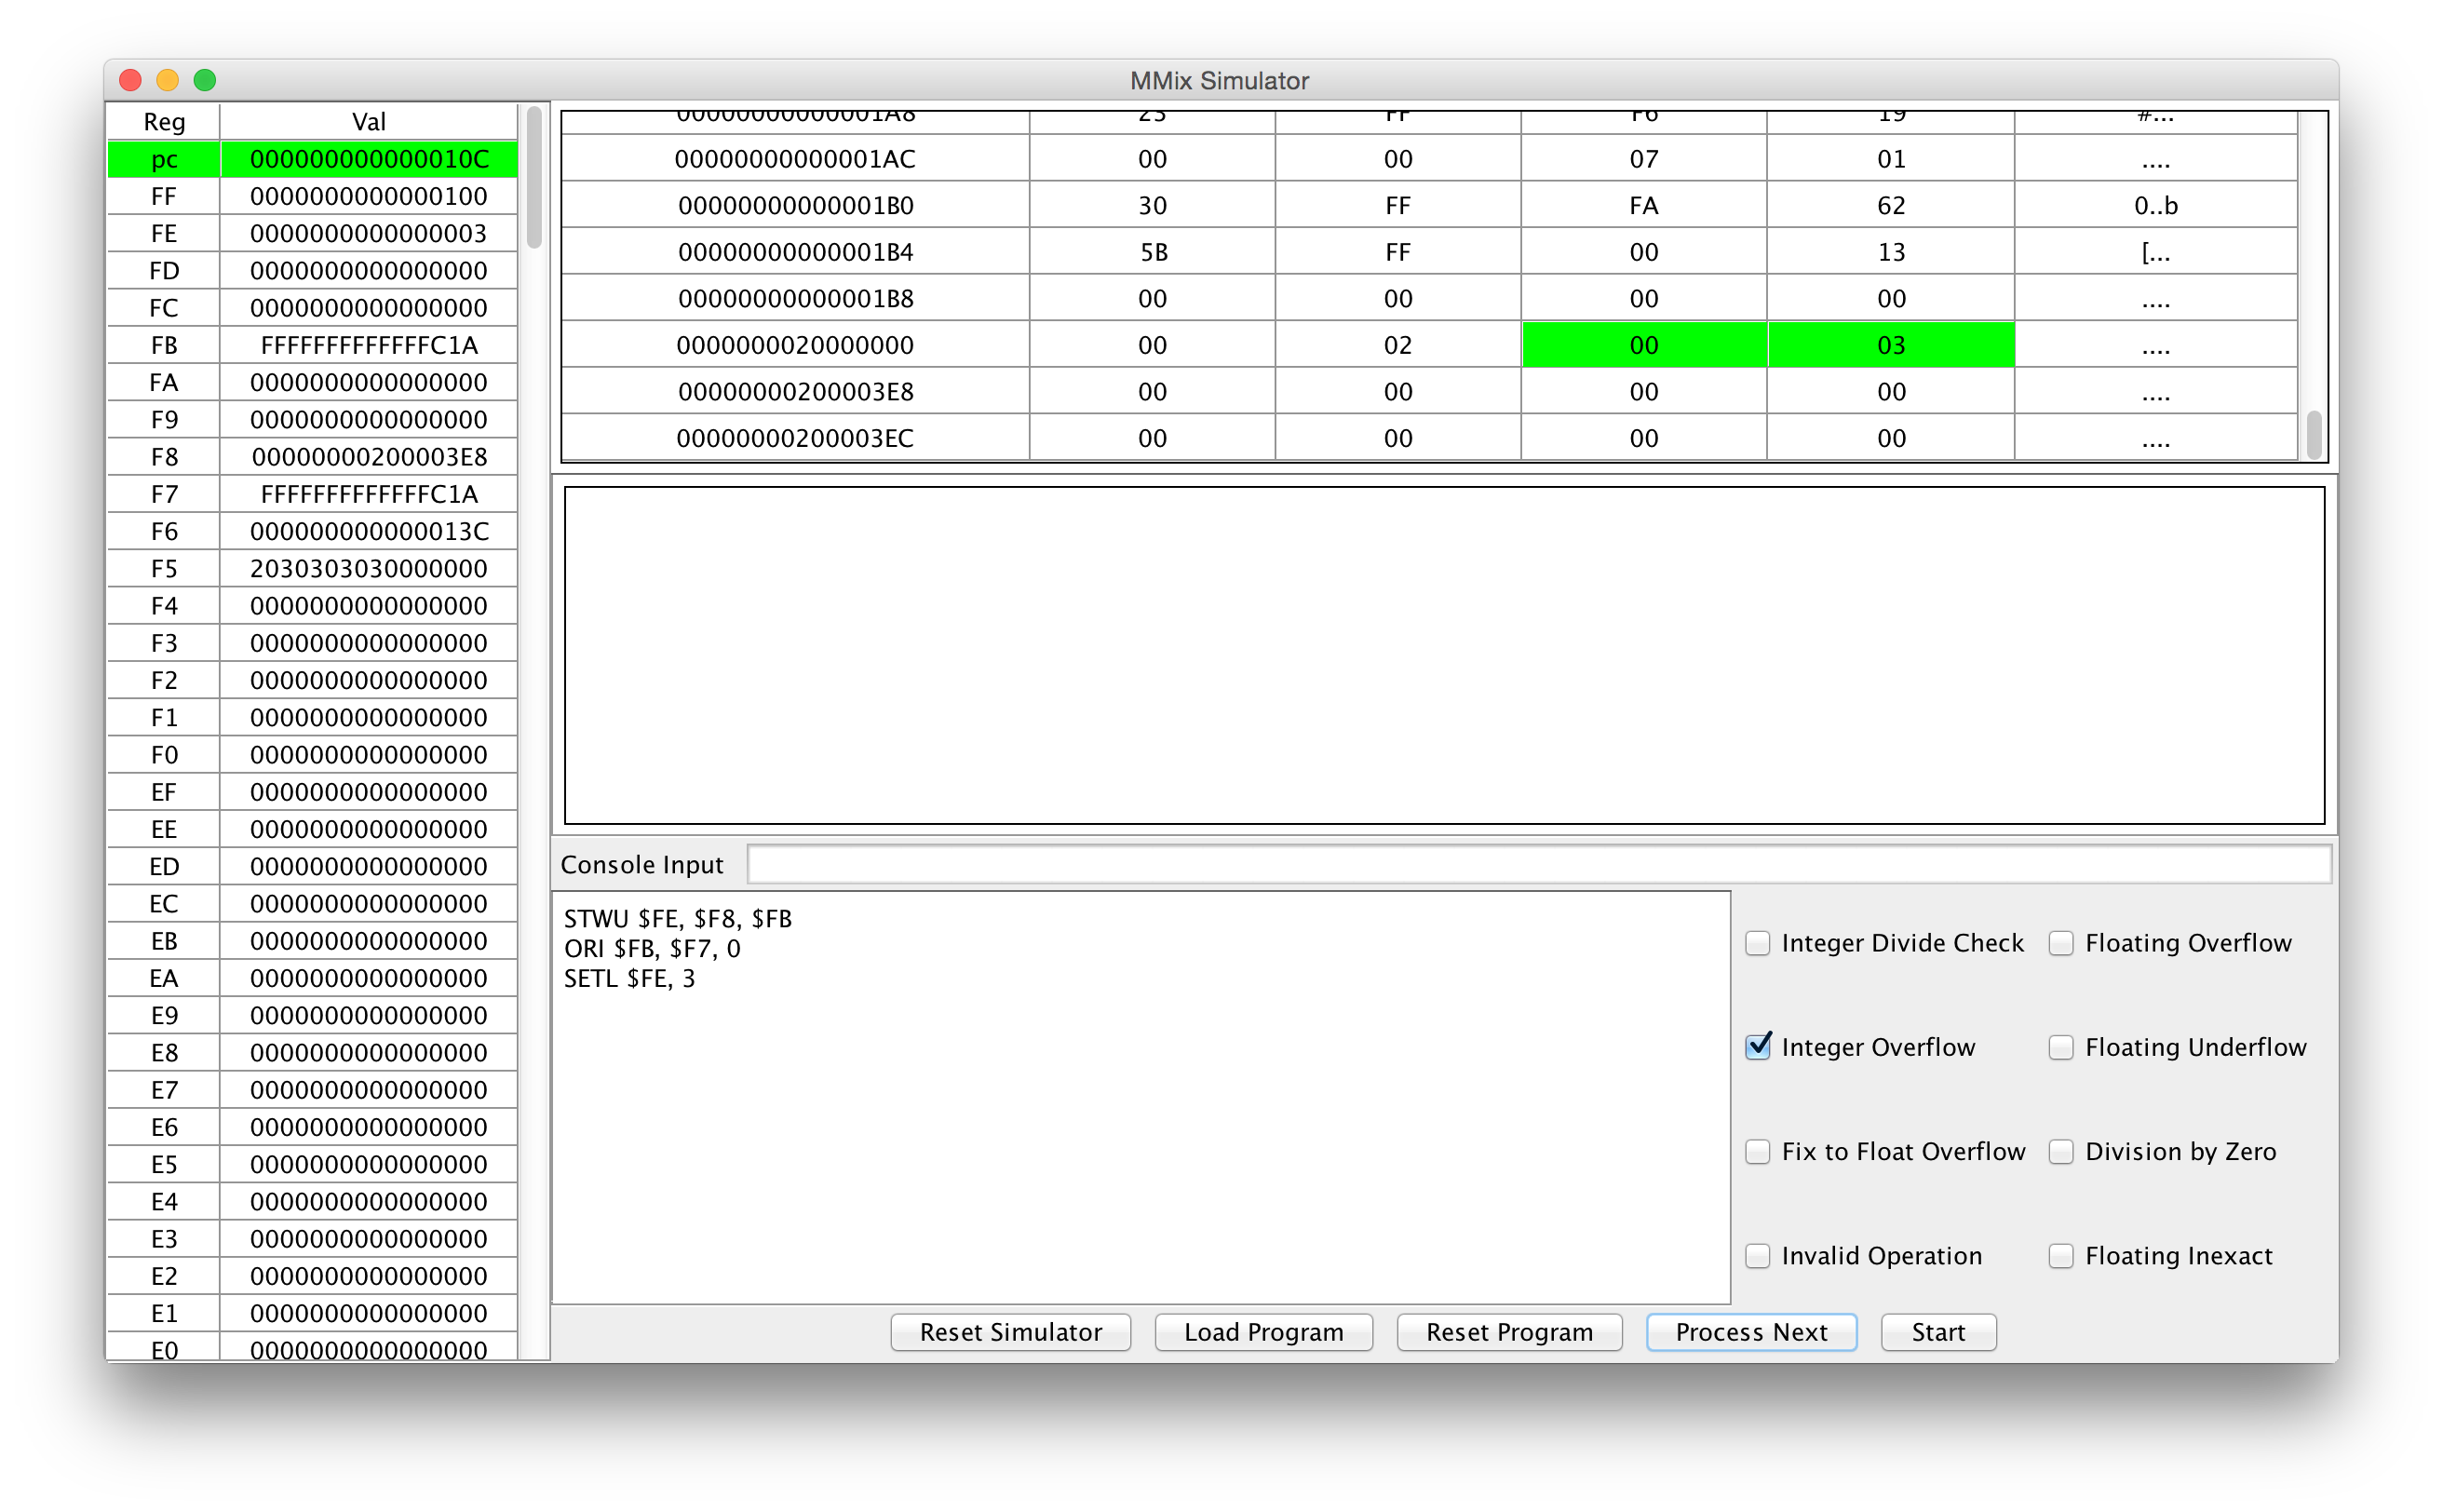
\includegraphics[width=\textwidth]{GUISample}
\caption{GUI Sample Screenshot}
\end{figure}

\section{User Interface Design}
\subsection{Console Panel}
\subsection{Controls Panel}
\subsection{Main State Panel}
\subsection{Memory Panel}
\subsection{Registers Panel}
\section[Asynchronous UI Programming with Actors]{Asynchronous User Interface Programming with Actors}
\section{Communication}
\section{Component Testing}
\chapter{Virtual Machine}
\section{Introduction}
Arhictecure of a computer  %% FIND QUOTATION
CPU, ALU, Memory, Secondary Storage, IO Devices

The virtaul machine we are developing will only consist of a CPU and memory.

The way that memory is organised can be considered a hierachy, to quote Aho et al\cite{dragon}
\begin{quotation}
A memory hierachy consists of several levels of storage with different sppeds and sizes, with the levels closest to the processor being the fastest but smallest... Memory hierarchies are found in all machines. A processor usually has a small number of registers consisting of hundres of bytes, several levels of caches containing kilobytes to megabytes, physical memory containing megabytes to gigabytes, and finally secondary storage that contains gigabytes and beyond.
\end{quotation}
For this project we will only be considering the physical memory and the registers.

\section{Memory}
Wyde

\begin{math}
M_2[0] = M_2[1] = M[0]M[1]
\end{math}

Tetra

\begin{math}
M_4[4k] = M_4[4k+1] = ... = M_4[4k+3] = M[4k]M[4k+1]...M[4k+3]
\end{math}

Octa

\begin{math}
M_8[8k] = M_8[8k+1] = ... = M_8[8k+7] = M[8k]M[8k+1]...M[8k+7]
\end{math}

\section{Registers}
An MMIX computer contains two distinct types of registers, 256 general purpose registers and 32 special purpose registers. A complete list of the special registers can be found in Figure~\ref{fig:spec_regs}

\begin{figure}[ht!]
\begin{center}
\begin{tabular}{ c l }
\head{Identifier} & \head{Description}\\
rA & Arithmetic Status Register\\
rB & Bootstrap Register\\
rC & Continuation Register\\
rD & Dividend Register\\
rE & Epsilon Register\\
rF & Failure Location Register\\
rG & Global Threshold Register\\
rH & Himult Register\\
rI & Interval Counter\\
rJ & Return-Jump Register\\
rK & Interrupt Mask Register\\
rL & Local Threshold Register\\
rM & Multiplex Mask Register\\
rN & Serial Number\\
rO & Register Stack Offset\\
rP & Prediction Register\\
rQ & Interrupt Request Register\\
rR & Remainder Register\\
rS & Register Stack Pointer\\
rT & Trap Address Register\\
rU & Usage Counter\\
rV & Virtual Translation Register\\
rW & Where Interrupted Register\\
rX & Execution Register\\
rY & Y Operand\\
rZ & Z Operand\\
rBB & Bootstrap Register\\
rTT & Dynamic Trap Address Register\\
rWW & Where Interrupted Register\\
rXX & Execution Register\\
rYY & Y Operand\\
rZZ & Z Operand\\
\end{tabular}
\end{center}
\caption{Special Registers}
\label{fig:spec_regs}
\end{figure}
rA Arithmetic Status Register

least signficant byte contains eight event bits. DVWIOUZX

\begin{center}
\begin{tabular}{ c l }
\head{Register} & \head{Description}\\
D & Integer Divide Check\\
V & Integer Overflow\\
W & Float-to-Fix Overflow\\
I & Invalid Operation\\
O & Floating Overflow\\
U & Floating Underflow\\
Z & Division by Zero\\
X & Floating Inexact\\
\end{tabular}
\end{center}

The next least significant byte contains eight ``enable'' bits with the same name DVWIOUZX and the same meanings.  

When an exceptional condition occurs, there are two cases: If the corresponding enable bit is 0, the corresponding event bit is set to 1; but if the corresponding enable bit is 1, MMIX interrupts its current instruction stream and execute a special ``exception handler''.  Thus, the event bits record exceptions that have not been ``tripped''.

This leaves six high order bytes.  At present, only  two of those 48 bits are defined. The two bits corresponding to 
\begin{math}
2^{17}
\end{math}
and 
\begin{math}
2^{16}
\end{math}
in rA specify a rounding mode, as follows: -

\begin{center}
\begin{tabular}{ c l }
00 & Round to the nearest\\
01 & Round off\\
10 & Round up\\
11 & Round down\\
\end{tabular}
\end{center}

\section{Central Processing Unit}
\section{Calling the Operating System}
\section{Communication}
\section{Component Testing}
\chapter{Simulator Application}
\section{Introduction}
%% HOW THE APPLICATION AS A WHOLE WORKS
\section{Integration Testing}
\subsection{Generate Prime Numbers Sample Application}
\chapter*{Conclusion}
\addcontentsline{toc}{chapter}{Conclusion}
\nocite{*}
\bibliographystyle{alpha}
\bibliography{bibtex}
\addcontentsline{toc}{chapter}{References}
\begin{appendices}
\noappendicestocpagenum
\addappheadtotoc 
\chapter{Source Code}
\section{Assembler}
\section{Graphical User Interface}
\section{Virtual Machine}
\chapter{Intermediate Assembler Representations}
\section{Definitions}
\section{Test Application}
\subsection{Sample Test MMIXAL Code}
The sample mmixal application I am using to test the system is taken from Fascile 1\cite{knuth:aocp2}.  The complete code listing is

\begin{CenteredBox}
\lstinputlisting{primes.mms}
\end{CenteredBox}
\subsection{Parsed Sample File}
The final version of the parsed source code for the test application is
\lstinputlisting[language=Haskell]{parsed_example.hs}
\end{appendices}
\clearpage
\addcontentsline{toc}{chapter}{Index}
\printindex
\end{document}

